\documentclass[12pt,letterpaper]{article}
\usepackage[latin1]{inputenc}
\usepackage[spanish]{babel}
\usepackage{graphicx}
\usepackage[left=2cm,right=2cm,top=2cm,bottom=2cm]{geometry}
\usepackage{graphicx} % figuras
\usepackage{subfigure} % subfiguras
\usepackage{float} % para usar [H]
\usepackage{amsmath}
\usepackage{txfonts}
\usepackage{stackrel} 
\usepackage{multirow}



\author{Fanny Clemente}
\title{Caratula}
\begin{document}



\author{Fanny Clemente}
\title{Caratula}

\begin{titlepage}
\begin{center}
\large{UNERSIDAD PRIVADA DE TACNA}\\
\vspace*{-0.025in}
\begin{figure}[htb]
\begin{center}

\includegraphics[width=8cm]{./figuras/logo}
\end{center}
\end{figure}
FACULTAD DE INGENIERIA\\
\vspace*{0.15in}
INGENIERIA DE SISTEMAS  \\

\vspace*{0.5in}
\begin{large}
TITULO:\\
\end{large}

\vspace*{0.1in}
\begin{Large}
\textbf{KID} \\
\end{Large}

\vspace*{0.3in}
\begin{Large}
\textbf{CURSO:} \\
\end{Large}

\vspace*{0.1in}
\begin{large}
BASE DE DATOS\\
\end{large}

\vspace*{0.3in}
\begin{Large}
\textbf{DOCENTE(ING):} \\
\end{Large}

\vspace*{0.1in}
\begin{large}
 Patrick Cuadros Quiroga\\
\end{large}


\vspace*{0.3in}
\rule{80mm}{0.1mm}\\
\vspace*{0.1in}
\begin{large}
Estudiante: \\
Fanny Luz Clemente Cruz \\
\end{large}
\end{center}

\end{titlepage}




 \tableofcontents
 \newpage
\listoftables
 \newpage
\listoffigures




\title{Un documento de Prueba} 
\author{fanny Cleente} 
\maketitle 
\section{Introducci�n} 
�Hola mundo \TeX !,  (escrito LaTeX en texto plano) es un sistema de composici�n de textos, orientado a la creaci�n de documentos escritos que presenten una alta calidad tipogr�fica. Por sus caracter�sticas y posibilidades, es usado de forma especialmente intensa en la generaci�n de art�culos y libros cient�ficos que incluyen, entre otros elementos, expresiones matem�ticas.



LaTeX es software libre bajo licencia LPPL.. 
\section{Tablas} 
\begin{table}[htbp]
\begin{center}
\begin{tabular}{|l|l|}
\hline
Pa�s & Ciudad \\
\hline \hline
Espa�a & Madrid \\ \hline
Espa�a & Sevilla \\ \hline
Francia & Par�s \\ \hline
\end{tabular}
\caption{Tabla  sencilla.}
\label{tabla:sencilla}
\end{center}
\end{table}


\begin{table}[htb]
\centering
\begin{tabular}{|l|l|}
\hline
\multicolumn{2}{|c|}{Europa} \\ \hline
Pa�s & Ciudad \\
\hline \hline
Espa�a & Madrid \\ \hline
Espa�a & Sevilla \\ \hline
Francia & Par�s \\ \hline
\end{tabular}
\caption{Tabla con 4 filas.}
\label{tabla:sencilla2}
\end{table}



\begin{table}[htb]
\centering
\begin{tabular}{|l|l|l|l|}
\hline
& \multicolumn{3}{c|}{Europa} \\
\cline{2-4}
& Ciudad & R�o & S�mbolo\\
\hline \hline
\multirow{3}{1cm}{Espa�a} & Madrid & Manzanares & Cibeles\\ \cline{2-4}
& Sevilla & Guadalquivir & Giralda\\ \cline{2-4}
& Zaragoza & Ebro & Pilar\\ \cline{1-4}
Francia & Par�s & Sena & Torre Eiffel\\ \cline{1-4}
\multirow{2}{1cm}{Italia} & Roma & T�ber & San Pedro\\ \cline{2-4}
& Mil�n & \multicolumn{1}{c|}{-} & Duomo\\ \cline{1-4}
\end{tabular}
\caption{Tabla con mas informaci�n .}
\label{tabla:final}
\end{table}


\begin{table}[htb]
\centering
\begin{tabular}{ c c c c c }
\hline
\multicolumn{5}{c}{Cuadro m�gico.}\\
\hline \hline
11 & 24 & 7 & 20 & 3\\
4 & 12 & 25 & 8 & 16\\
\cline{2-2}
17 & \multicolumn{1}{|c|}{5} & 13 & 21 & 9\\
\cline{2-2} \cline{4-5}
10 & 18 & 1 & \multicolumn{1}{|c}{14} & \multicolumn{1}{c|}{22}\\
\cline{4-5}
23 & 6 & 19 & 2 & 15\\
\hline
\end{tabular}
\caption{Tabla de numeros.}
\label{tabla:sinlineas}
\end{table}
% cline{1-2} = crea una l�nea horizontal entre la columna 1 y la 2. 


\begin{table}[htb]
\centering
\begin{tabular}{|c|r@{.}l|}
\hline
\multicolumn{3}{|c|}{N�meros decimales} \\
\hline
A & 2 & 501 \\
\hline
B & 15 & 4 \\
\hline
C & 3700 & 25 \\
\hline
\end{tabular}
\caption{N�meros ajustados en el punto decimal.}
\label{tabla:ajustepunto}
\end{table}

\begin{table}[H]
\centering
\begin{tabular}{p{2cm} p{5cm}}
\hline
Autor & Poema \\
\hline \hline
Espronceda & Con diez ca�ones por banda, viento en popa, a toda vela, no corta el mar, sino vuela un velero bergant�n... \\
\hline
B�cquer & Volver�n las oscuras golondrinas, en tu balc�n sus nidos a colgar, y otra vez con el ala, a sus cristales jugando llamar�n... \\
\hline
\end{tabular}
\caption{Autores espa�oles.}
\label{tabla:autores}
\end{table}









\newpage

\section{f�rmulas} 
\subsection{Integrales}
formula 1:
$$ \frac{\pi}{4} = \int_0^1 \frac{1}{1+x^2} dx $$ 
Formula 2:
\begin{equation}
  w = \sum_{i=1}^{n} (x_{i}+y_{i})^{2}
\end{equation}\\

\begin{equation}
y = \int \limits_{x=0}^{x=2 \pi + 10} f(x) \cdot dx 
\end{equation}\\


\begin{equation}
y = \int \limits_{x=0}^{x=2 \pi + 10} \!\!\!\!\!\!\! f(x) \cdot dx
\end{equation}\\



\begin{equation}
y = \iint f(x) = \iiint g(x) = \idotsint h(x) 
\end{equation}\\

\begin{equation}
z = \int _{y=a}^{y=b} \int _{x=g(y)}^{x=h(y)} f(x) \cdot dx \cdot dy
\end{equation}\\
\begin{equation}
y = \dfrac{\int_{x=0}^{x=2 \pi + 10} f(x) \cdot dx}{g(x)}
\end{equation}

\begin{equation}
\oint_L = \oiint_A = \oiiint_V
\end{equation}
\subsection{Relaciones Quimicas}

\begin{equation} \label{reac:A2B}
A \rightarrow B
\end{equation}


\begin{equation}
A_{2}^{+} \rightarrow B^{+}
\end{equation}

\begin{equation}
^{1}B \rightleftarrows 2 \cdot C
\end{equation}

\begin{equation}
C \xrightarrow[a]{b} D
\end{equation}

\begin{equation} 
D \rightarrow E\uparrow + F\downarrow
\end{equation}

\begin{equation}
\mathrm{NO_{3}^{-} + S_{2}O_{7}^{2-} \xrightarrow[T\uparrow]{H^{+}} NO_{2}^{+} + 2 SO_{4}^{2-}}
\end{equation}

\begin{equation}
A + B \stackbin[T_1]{P_1}{=} C + D
\end{equation} \\
\subsection{fracciones}

Ejemplo con fracciones:  $z = \frac{1}{x} + 4$
\begin{equation}
 z = \frac{1}{x} + 4
\end{equation}

Ejemplo con fracciones:  $z = \dfrac{1}{x} + 4$
\begin{equation}
 z = \dfrac{1}{x} + 4
\end{equation}

Ejemplo con fracciones:  $z = \tfrac{1}{x} + 4$
\begin{equation}
 z = \tfrac{1}{x} + 4
\end{equation}

\begin{equation}
 z = \cfrac{1}{2 + \cfrac{1}{\cfrac{z}{1+y}}}
\end{equation}



\newpage

\section{Graficos} 

\begin{figure}[htb]
\centering
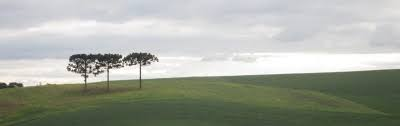
\includegraphics[width=0.8\textwidth]{./figuras/horizonte}
\caption{Mar Atl�ntico.} \label{fig:horizonte}
\end{figure}


\begin{figure}[htbp]
\centering
\subfigure[Starks]{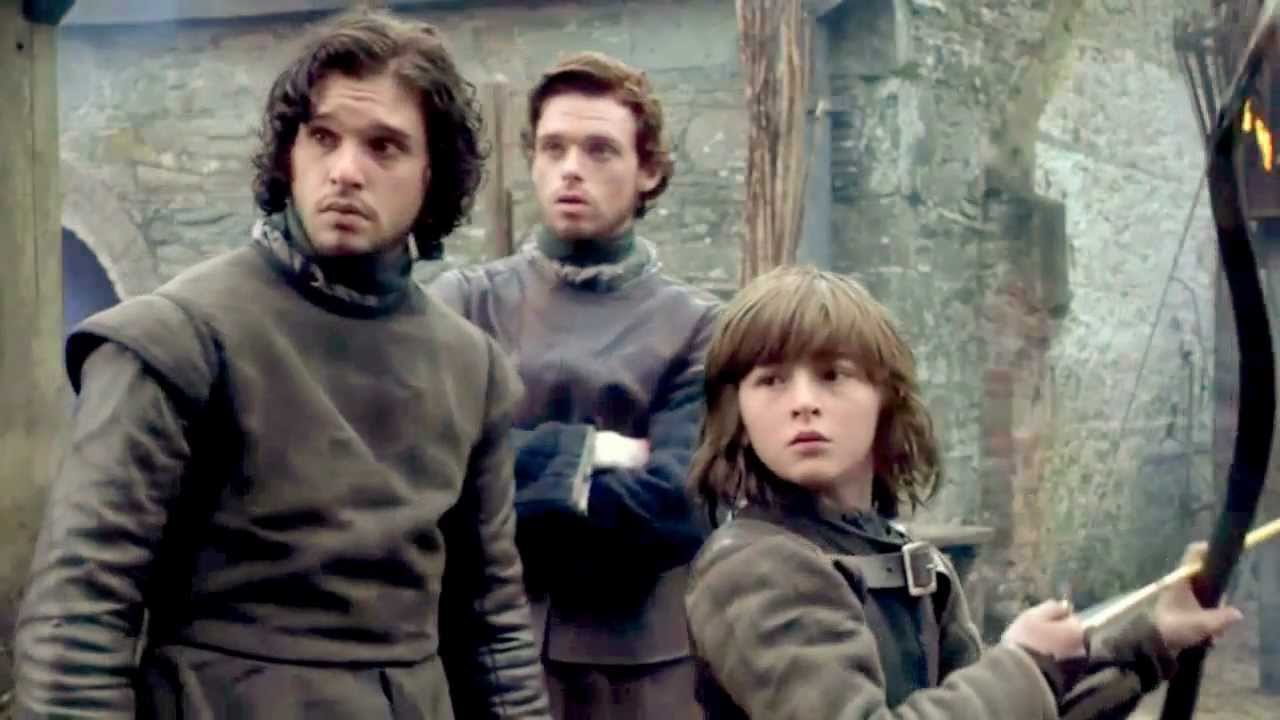
\includegraphics[width=40mm]{./figuras/starks1}}
\subfigure[Arya y Reeds]{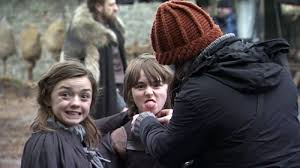
\includegraphics[width=40mm]{./figuras/starks2}}
\subfigure[Lannisters]{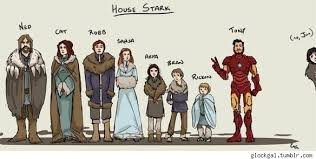
\includegraphics[width=80mm]{./figuras/lannisters}}
\caption{Legos.} \label{fig:lego}
\end{figure}



\begin{figure}[htb]
\centering
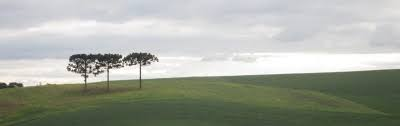
\includegraphics[width=0.8\textwidth]{./figuras/horizonte}
\caption{Mar Atl�ntico.} \label{fig:horizonte}
\end{figure}


\newpage
\section{Bibliografia} 
@ARTICLE{Alfonso2010a,
author = {M. Alfonso and B. Bernardo and C. Carlos and D. Domingo},
title = {El problema de los gatos y los perros},
journal = {Mascotas},
year = {2010},
volume = {50},
pages = {112-115}
}

@ARTICLE{Alfonso2010b,
author = {M. Alfonso and M. Marta and N. Nuria},
title = {Mi viaje a {EEUU}},
journal = {Revista de viajes},
year = {2010},
volume = {14},
pages = {50-56}
}

@ARTICLE{Patricio2011,
author = {A. Patricio},
title = {Una estrella rosa en el fondo del mar},
journal = {El mar},
year = {2011},
volume = {3},
pages = {1071-1090}
}

@ARTICLE{Zacarias2009,
author = {R. Zacarias and G. Graciela},
title = {�{C}u�l te gusta m�s?},
journal = {Flores},
year = {2009},
volume = {5},
pages = {45-49}
}



\end{document}
